\documentclass[11pt, a4paper, twoside]{article}   	% use "amsart" instead of "article" for AMSLaTeX format

\usepackage{geometry}                		% See geometry.pdf to learn the layout options. There are lots.
\usepackage{pdfpages}
\usepackage{caption}
\usepackage{minted}
\usepackage[german]{babel}			% this end the next are needed for german umlaute
\usepackage[utf8]{inputenc}
\usepackage{color}
\usepackage{graphicx}
\usepackage{titlesec}
\usepackage{fancyhdr}
\usepackage{lastpage}
\usepackage{hyperref}
% http://www.artofproblemsolving.com/wiki/index.php/LaTeX:Symbols#Operators
% =============================================
% Layout & Colors
% =============================================
\geometry{
   a4paper,
   total={210mm,297mm},
   left=20mm,
   right=20mm,
   top=20mm,
   bottom=30mm
 }	

\definecolor{myred}{rgb}{0.8,0,0}
\definecolor{mygreen}{rgb}{0,0.6,0}
\definecolor{mygray}{rgb}{0.5,0.5,0.5}
\definecolor{mymauve}{rgb}{0.58,0,0.82}

\setcounter{secnumdepth}{4}


% the default java directory structure and the main packages
\newcommand{\srcDir}{/src/main/java}
% =============================================
% Code Settings
% =============================================
\newenvironment{code}{\captionsetup{type=listing}}{}
\newmintedfile[javaSourceFile]{java}{
	linenos=true, 
	frame=single, 
	breaklines=true, 
	tabsize=2,
	numbersep=5pt,
	xleftmargin=10pt,
	baselinestretch=1,
	fontsize=\footnotesize
}
\newmintinline[inlineJava]{java}{}
\newminted[javaSource]{java}{
	breaklines=true, 
	tabsize=2,
	autogobble=true,
	breakautoindent=false
}
\newmintedfile[xmlSourceFile]{xml}{
	linenos=true, 
	frame=single, 
	breaklines=true, 
	tabsize=2,
	numbersep=5pt,
	xleftmargin=10pt,
	baselinestretch=1,
	fontsize=\footnotesize
}
\newmintedfile[propertiesFile]{properties}{
	linenos=true, 
	frame=single, 
	breaklines=true, 
	tabsize=2,
	numbersep=5pt,
	xleftmargin=10pt,
	baselinestretch=1,
	fontsize=\footnotesize
}
\newmintedfile[sqlFile]{sql}{
	linenos=true, 
	frame=single, 
	breaklines=true, 
	tabsize=2,
	numbersep=5pt,
	xleftmargin=10pt,
	baselinestretch=1,
	fontsize=\footnotesize
}
% =============================================
% Page Style, Footers & Headers, Title
% =============================================
\title{Übung 3}
\author{Thomas Herzog}

\lhead{Übung 3}
\chead{}
\rhead{
\includegraphics[scale=0.10]{FHO_Logo_Students.jpg}}

\lfoot{S1310307011}
\cfoot{}
\rfoot{ \thepage / \pageref{LastPage} }
\renewcommand{\footrulewidth}{0.4pt}
% =============================================
% D O C U M E N T     C O N T E N T
% =============================================
\pagestyle{fancy}
\begin{document}
\setlength{\headheight}{15mm}
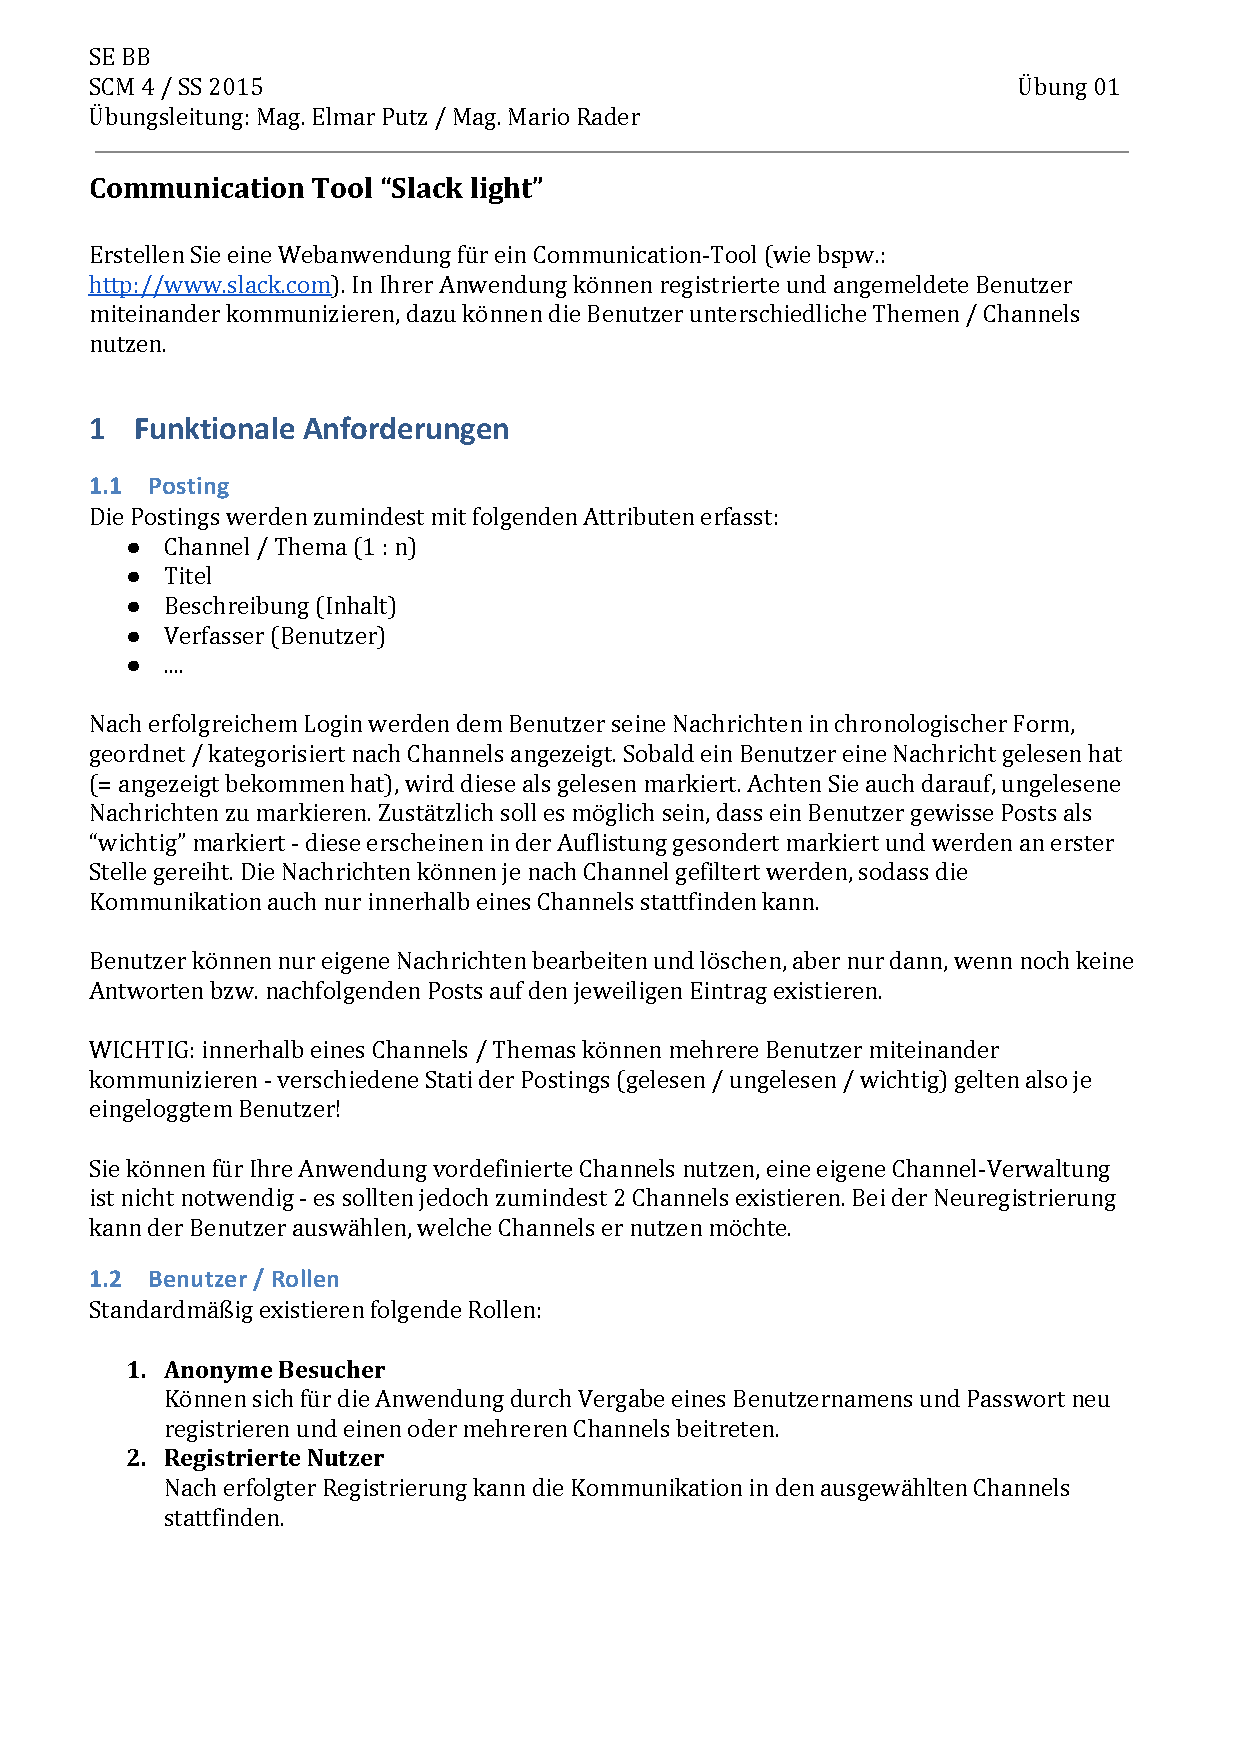
\includepdf[pages={1,2,3}]{scm4-2015-uebung01-communication-list.pdf}
{\color{myred}
	\section
		{Kommunikationstool 'Slack Light'}
}

% =============================================
% Idea section
% =============================================
\subsection{Datenbank}
Folgende Abbildung zeigt das ER Diagramm des Datenmodells für das Kommunikationstool "Slack light". \
\begin{figure}[h]
	\centering
	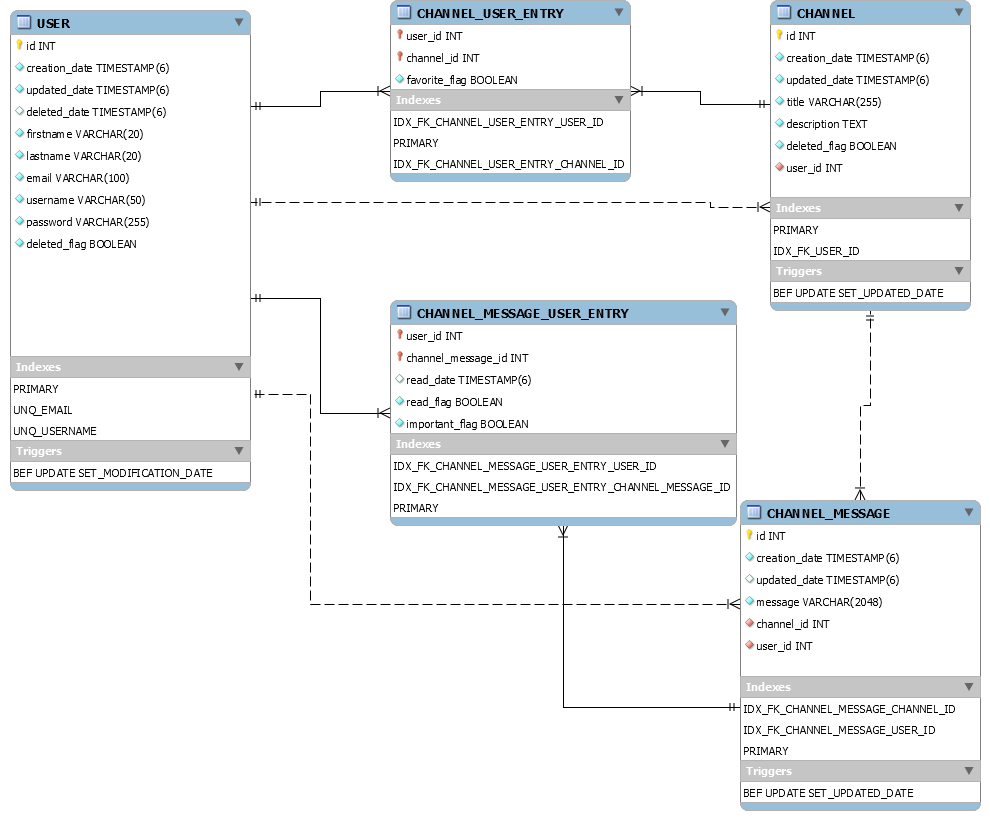
\includegraphics[scale=0.5]{images/er-model.PNG}
	\caption
	{ER-Modell}
\end{figure}

\newpage
\subsection{Applikationsarchitektur}
Folgender Abschnitt beschreibt die Architektur der Applikation.\\
Die Applikation ist in zwei Haupt PHP Dateien aufgeteilt über die alle Request gehandelt werden:
\begin{enumerate}
	\item \textbf{index.php:} \\
	All offenen Ressourcen wie Login und Registrierung 
	\item \textbf{start.php:} \\
	Alle geschützten Ressourcen, die einen Login erfordern.
\end{enumerate}
Diese Dateien sowie alle *.css, *.js Dateien sowie Images sind in einem public Verzeichnis zusammengefasst und können ohne Zugriffskontrolle abgerufen werden.\\
Alle anderen angezeigten Seiten werden über das Templating Tool \textbf{Twig} generiert und werden über die beiden PHP Dateien index.php oder start.php and den Client übermittelt. Dadurch ist kein direkter Zugriff auf diese Dateien möglich.
\\\\
Folgende Abbildung illustriert die Architektur der Applikation beziehungsweise den Ablauf eines Requests. \\
\begin{figure}[h]
	\centering
	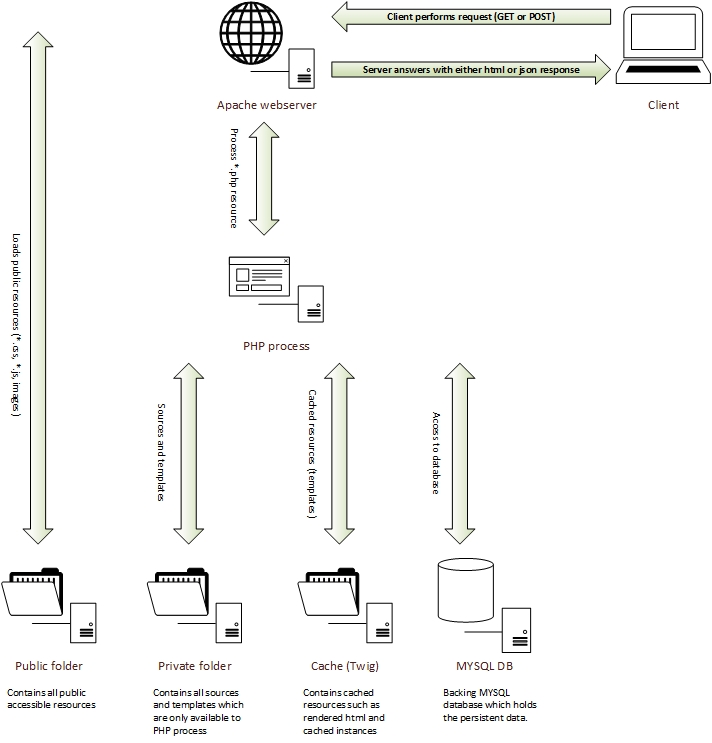
\includegraphics[scale=0.725]{images/Infrastructure.JPG}
	\caption
	{Applikationsarchitektur}
\end{figure}

\newpage 
Die Applikation wurde in 3 Ebenen unterteilt, wobei nicht alle Ebenen nach außen frei zugänglich sind.\\
\begin{enumerate}
	\item \textbf{public/*} \\
	Enthält alle öffentlich und ohne Einschränkung zugängliche Ressourcen. Diese Ressourcen sind direkt über den Webserver zugänglich und müssen nicht von einem PHP Prozess provided werden. Diese sind z.B.: Javascript-, CSS-, Image-Dateien oder die beiden Hauptseiten index.php und start.php (erfordert eingeloggten Benutzer). 
	\item \textbf{source/*} \\
	Alle geschützten Ressourcen wie die PHP Sources und die Twig Templates. Sie sind nur über den PHP Prozess und Source in index.php und start.php erreichbar. Dadurch sind die Sources von außen abgeschirmt, wobei der Webserver diese Verzeichnisse von einem externen zugriff zu schützen hat.
	\item \textbf{cache/*}\\
	Enthält die kompilierten Twig Templates sowie die gerenderten Html-Dateien, somit müssen diese nicht bei jeder Verarbeitung neu kompiliert oder gerendert werden. Der Code entschiedet hierbei ob ein erneutes Rendern erforderlich ist oder nicht.
\end{enumerate}
Es werden zwei externe Libraries verwendet, die zwar über composer geladen wurden aber über einen eigenen Autoloader innerhalb des PHP Prozess geladen werden.
\begin{enumerate}
	\item \textbf{Twig:}\\
	Hierbei handelt es sich um eine Template Library, die dazu verwendet wird um die Html-Dateien für den Client aufzubereiten. Hierzu wird ein Assoziativen Array mit Parametern befüllt, welche innerhalb der Twig-Template-Engine verarbeiten werden um das Html zu produzieren. Dabei ist kein PHP Source in den Html-Dateien enthalten, was meiner Meinung nach die Übersichtlichkeit erhöht, den der dynamische Content wird innerhalb des PHP Codes aufbereitet und nur die Ausgabeparameter an die Twig-Template-Engine weitergereicht.
	\item \textbf{Stash:}\\
	Hierbei handelt es sich um eine Caching Library, welche dazu verwendet wird um die gerenderten Html-Dateien zu cachen, damit diese nicht immer neu verarbeitet werden müssen. Im PHP Code wird entschieden ob eine Html-Datei neu gerendert werden soll oder ob diese aus den Cache genommen werden soll.
\end{enumerate}
\newpage

\subsection{Tests}
Folgend sind die Tests für die Applikation angeführt.
\subsubsection{Benutzerregistrierung}
Folgend sind die Tests für die Benutzerregistrierung angeführt.\\\\
Folgender Test zeigt die angewendete Client Validierung über Bootstrap-Form-Validation Plugin. 
\begin{figure}[h]
	\centering
	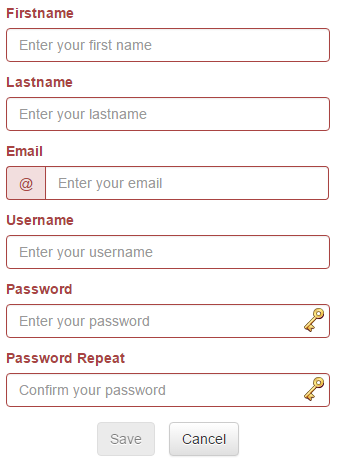
\includegraphics[scale=0.5]{images/registration_client_validation_full.PNG}
	\caption
	{Bootstrap Form Validation}
\end{figure}\\\\
Neben der Required Validerung erfolgt auch eine Validierung auf eine syntaktisch gültige E-Mail Adresse.
\begin{figure}[h]
	\centering
	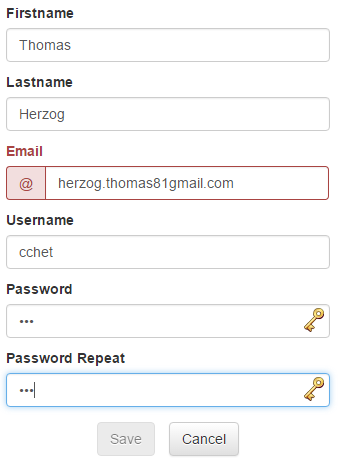
\includegraphics[scale=0.5]{images/registration_client_validation_email.PNG}
	\caption
	{Bootstrap Form Validation E-Mail}
\end{figure}
\newpage
Wenn eine E-Mail bereits von einem Benutzer verwendet wird, dann wird dies serverseitig Validiert und an eine Fehlermeldung an den Client übermittelt.
\begin{figure}[h]
	\centering
	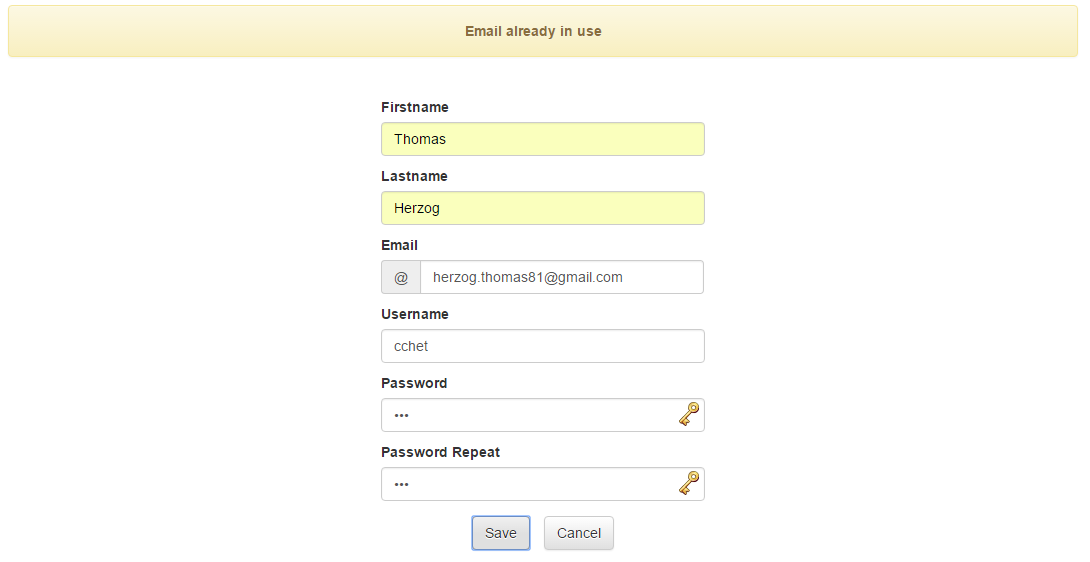
\includegraphics[scale=0.4]{images/registration_server_validation_email.PNG}
	\caption
	{Serverseitige E-Mail Validierung}
\end{figure}\\\\
Wenn ein Benutzername bereits von einem aktiven Benutzer verwendet wird, dann wird dies serversetig validiert und eine Fehlermeldung and den Client übermittelt.
\begin{figure}[h]
	\centering
	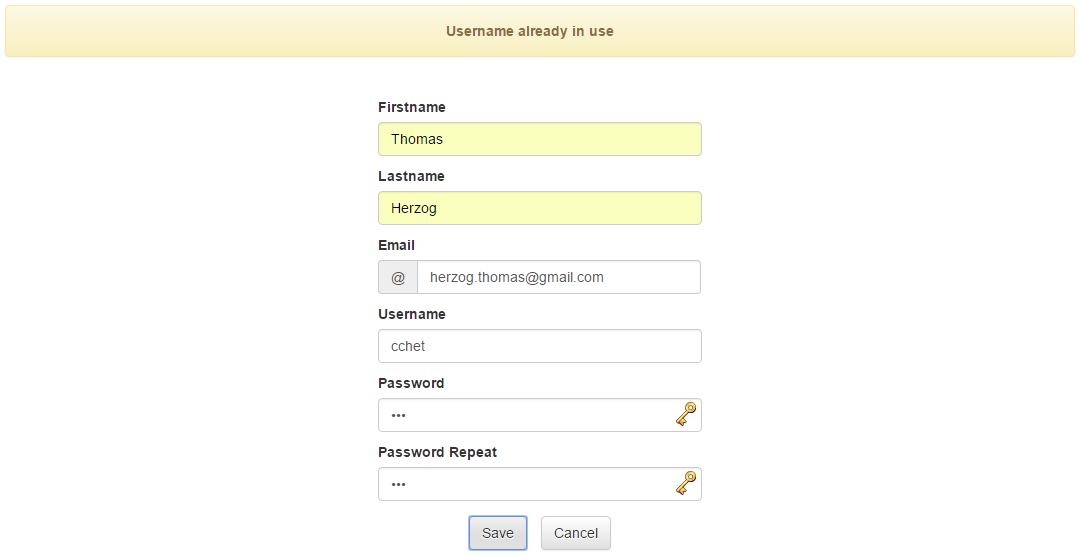
\includegraphics[scale=0.4]{images/registration_server_validation_username.PNG}
	\caption
	{Serverseitige Benutzernamen Validierung}
\end{figure}
\newpage
Nach der erfolgreichen Registrierung eines Benutzers wird eine Erfolgsmeldung angezeigt, wobei nach einigen Sekunden automatisch auf die Login Seite weitergeleitet wird, obwohl ebenfalls eine Button zur Verfügung steht, der auf die Login Seite wechselt sollte das automatische Weiterleiten nicht funktionieren.
\begin{figure}[h]
	\centering
	
\includegraphics[scale=0.6]{images/registration_success.PNG}
	\caption
	{Registrierung erfolgreich}
\end{figure}\\\\



\end{document}  